\newcommand{\circscale}{.85}
\begin{tikzpicture}

	\begin{scope}[scale=\circscale,
		nod/.style={align=center,fill=white, opacity=.75, text opacity=1,rounded corners=6 pt,inner sep=1.5 pt},
		setts/.style={color=black,very thick, ->}
		]
		% Unscaled scale=.2
		% PMF w/ friction
		\node at (1.5 cm, 0){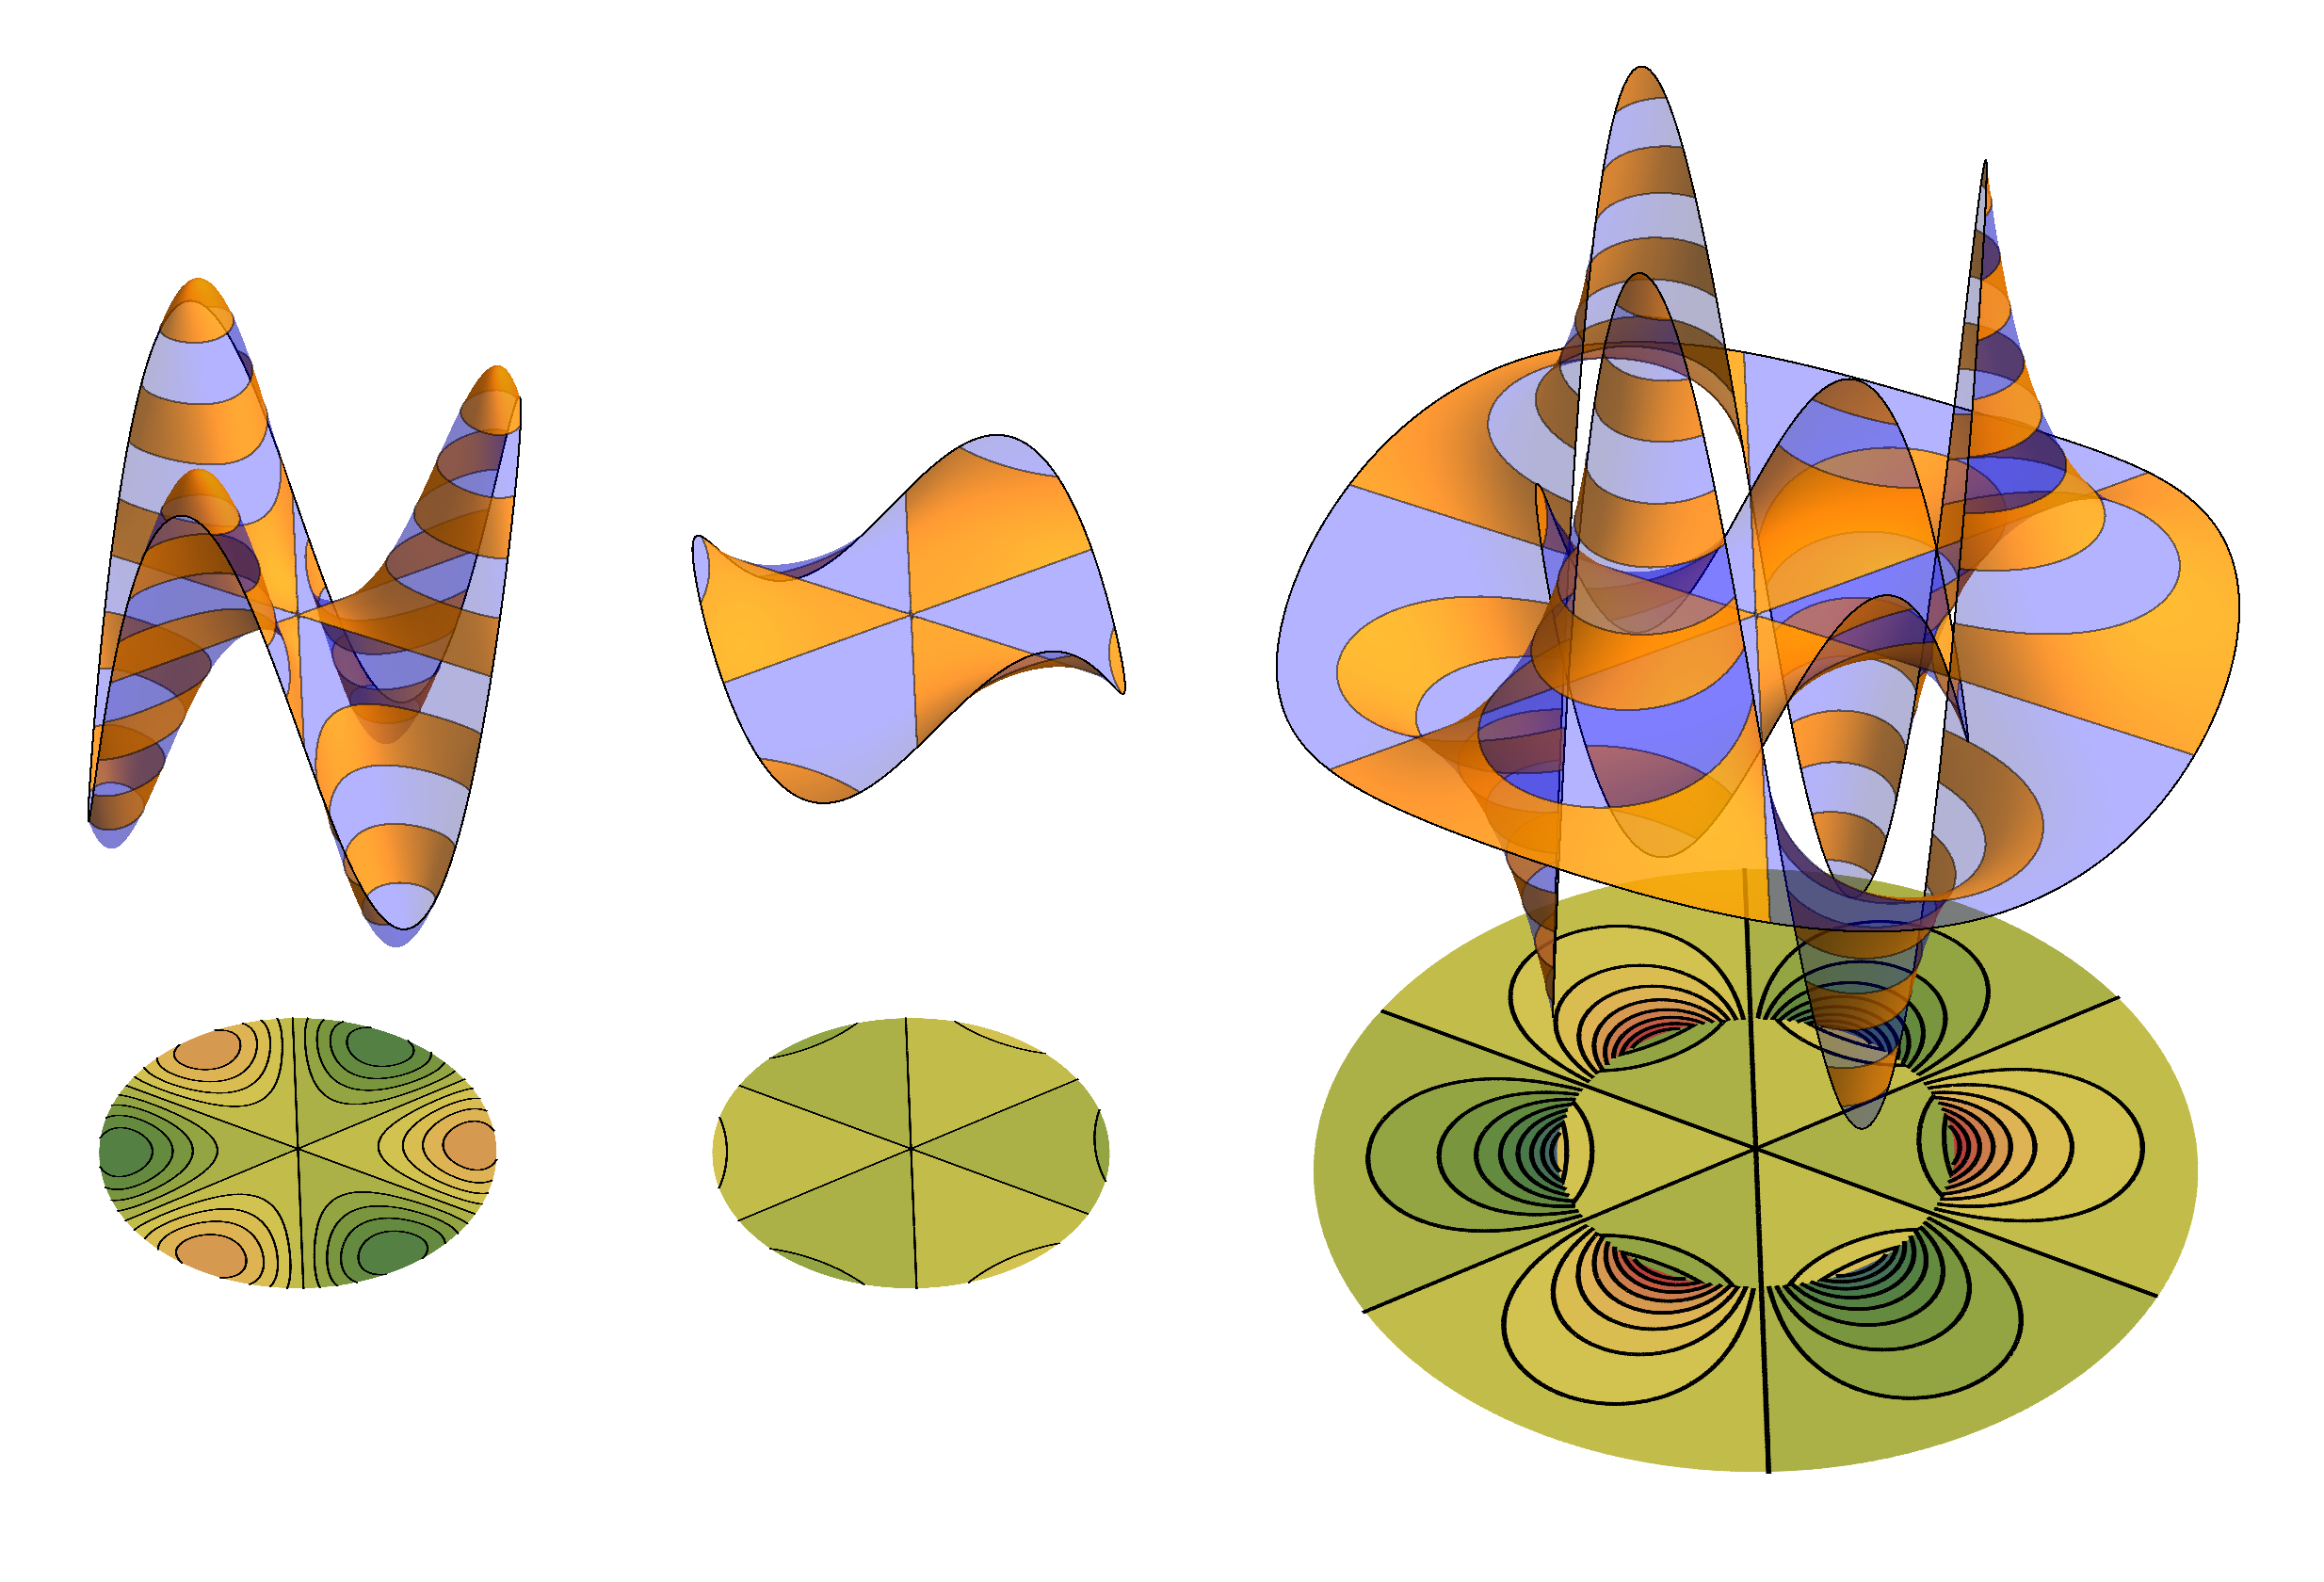
\includegraphics[scale=.17, clip=true, trim=35cm 0 0 0]{Poster/Circle_PMF.png}};
		% PMF w/o friction
		\node at (-4 cm, 0){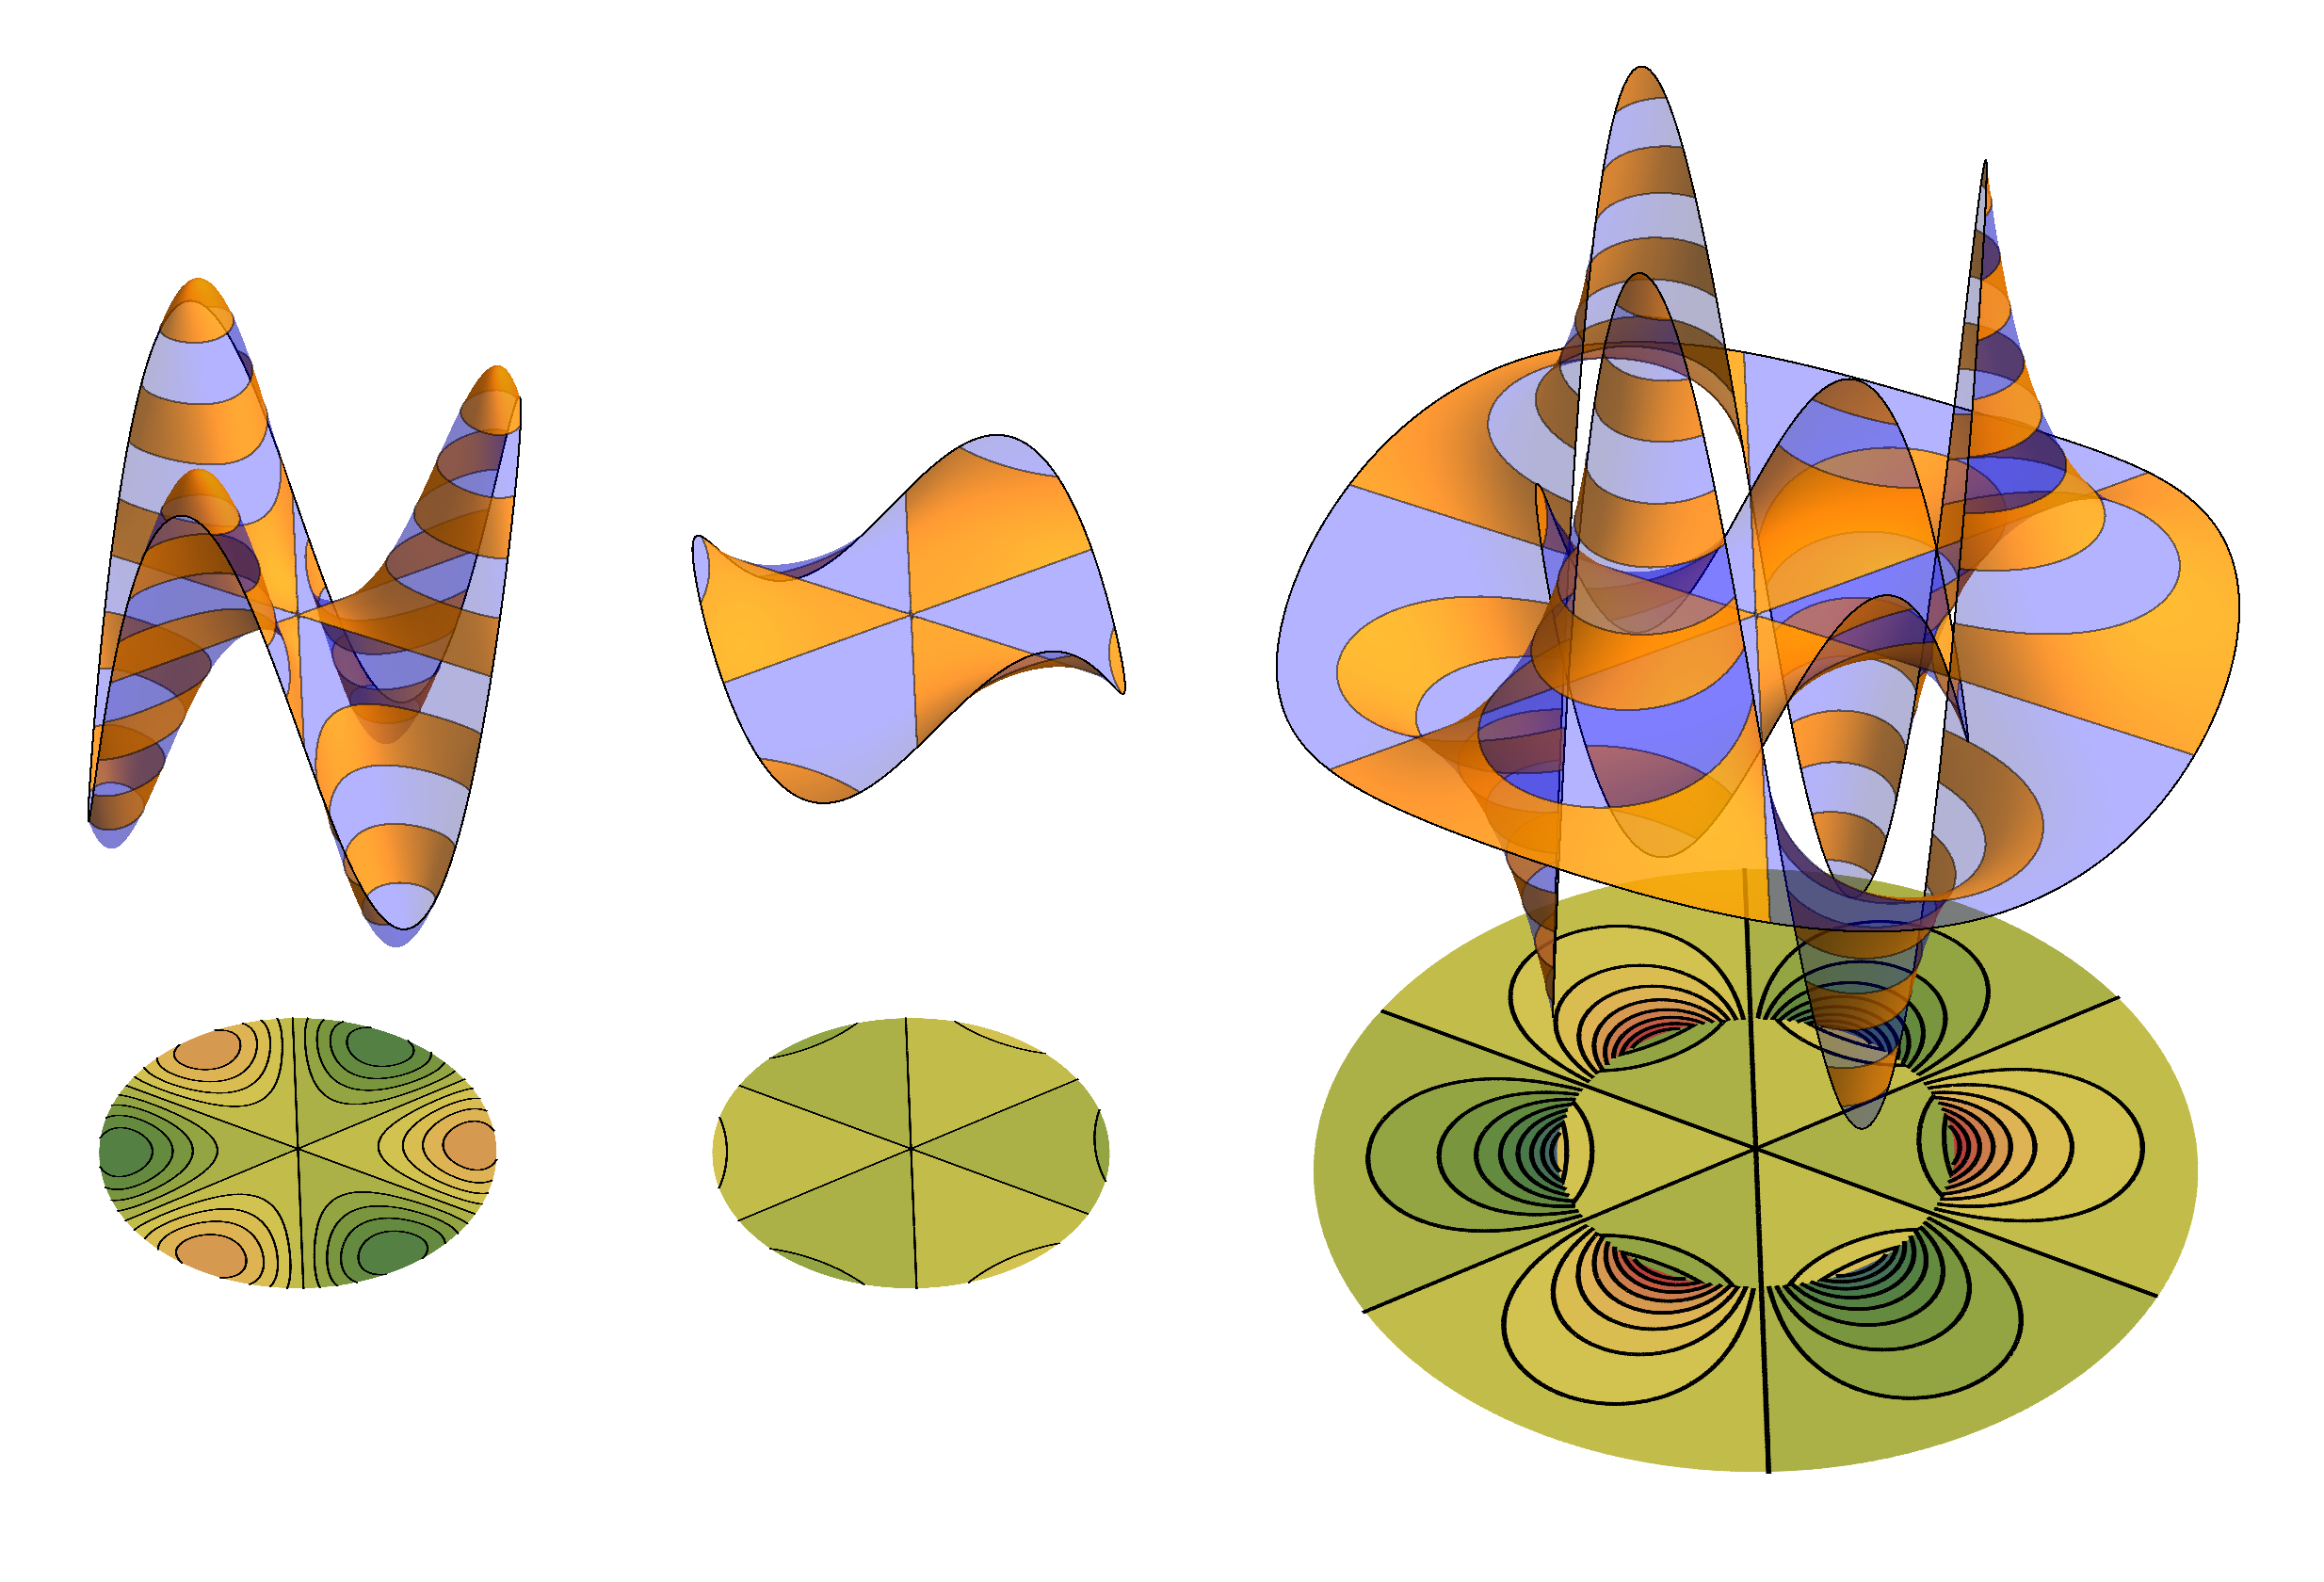
\includegraphics[scale=.17, clip=true, trim=15cm 0 30cm 0]{Poster/Circle_PMF.png}};
		% Color bar
		\node at (7 cm,-0.5 cm){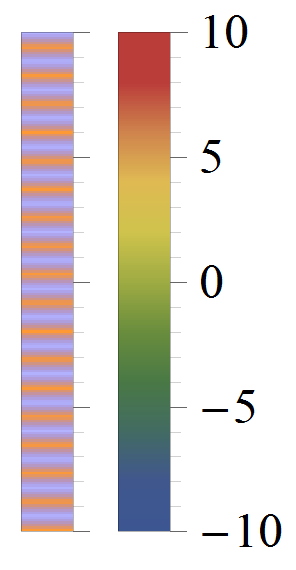
\includegraphics[scale=\circscale]{Poster/Circle_PMF_Bar.png}};

		% PMF labels
		\node at (-4,4)   [nod]	{\textbf{Fixed} \\ \textbf{Boundaries}};
		\node at (1.5cm,4) [nod]	{\textbf{Sliding} \\ \textbf{Against Friction}};
		\node at (6.8cm,2.5cm)[nod]	{\textbf{Pseudomagnetic} \\ \textbf{Field (T)}};

		%Scale bar
		\draw[draw=black,ultra thick, xshift=4cm, yshift=-3.5cm] (0,0) -- node[anchor=south] {100 nm}(1.09 cm, 0);
	\end{scope}

	\newcommand{\topthick}{.3 cm}
	\newcommand{\botthick}{8 cm}
	\newcommand{\basethick}{2 cm}
	\newcommand{\edge}{12 cm}
	\newcommand{\radius}{5 cm}
	\newcommand{\srad}{.5 cm}
	\newcommand{\grup}{0 cm}
	\begin{scope}[scale=0.19,xshift=6cm,yshift=-35cm,
		sio2/.style={fill=blue!50!white,draw=none},
		siedge/.style={draw=black!50!white}]

		%Image of a hole (top view)
		\begin{scope}[xshift=0 cm,yshift=10 cm]
			\node at (0,0) {
\includegraphics[scale=0.93,clip=true,trim=1.32cm .45cm 1.32cm .45cm]{Poster/SB03-2.jpg}};
		\end{scope}
		
		%The SiO2
		\filldraw[sio2] (-\edge,0) -- (-\radius, 0) -- (-\radius, -\topthick) -- (-\edge, -\topthick);
		\filldraw[sio2] (\edge,0) -- (\radius, 0) -- (\radius, -\topthick) -- (\edge, -\topthick);
		
		%The Si
		\fill[fill=black!20!white]
			(-\edge,-\topthick) -- (-\radius,-\topthick) 
			\foreach \i in {0,...,15}
				{-- (-\radius, -\topthick-\i*\srad) .. controls (-\radius-\srad/4, -\topthick-\srad/4-\i*\srad) and (-\radius-\srad/4, -\topthick-3*\srad/4-\i*\srad) ..
				(-\radius,-\topthick-\srad-\i*\srad) }
			-- (-\radius, -\topthick-\botthick) node[anchor=south west] {$P_0$} -- 
			(\radius, -\topthick-\botthick) 
			\foreach \j in {15,14,...,0}
				{-- (\radius, -\topthick-\srad-\j*\srad) .. controls (\radius+\srad/4, -\topthick-3*\srad/4-\j*\srad) and (\radius+\srad/4, -\topthick-\srad/4-\j*\srad) ..
				(\radius,-\topthick-\j*\srad) }
			 -- (\edge, -\topthick) -- 
			(\edge, -\topthick-\botthick-\basethick) -- (-\edge, -\topthick-\botthick-\basethick) [draw=none]-- cycle ;
		
		\draw[siedge](-\edge,-\topthick) --(-\radius,-\topthick);
		\foreach \i in {1,...,16}
			\draw[yshift=-1*(\i-1)*\srad,siedge] (-\radius, -\topthick) .. controls (-\radius-\srad/4, -\topthick-\srad/4) and (-\radius-\srad/4, -\topthick-3*\srad/4) ..
				(-\radius,-\topthick-\srad);
		\draw[siedge] (-\radius, -\topthick-\botthick) -- (\radius, -\topthick-\botthick);
		\draw[siedge] (\radius, -\topthick) -- (\edge, -\topthick);
		\foreach \i in {1,...,16}
			\draw[yshift=-1*(\i-1)*\srad,siedge] (\radius, -\topthick) .. controls (\radius+\srad/4, -\topthick-\srad/4) and (\radius+\srad/4, -\topthick-3*\srad/4) ..
				(\radius,-\topthick-\srad);
		
		%The Graphene on the top
		\draw[thick] (-\edge,\grup) -- (-\radius,\grup) node[anchor=south west]{$P>P_0$}  parabola bend (0,-.7 cm)  (\radius,\grup) -- (\edge,\grup);
		
		%Dashed lines
		\draw[color=black!80!white,dashed] (-\radius,\grup+.5cm) -- (-\radius,\grup+26 cm);
		\draw[color=black!80!white,dashed] (\radius,\grup+.5cm) -- (\radius,\grup+26 cm);
	\end{scope}
\end{tikzpicture}